\section{La cardinalità del numerabile}

\begin{definition}[Numerabilità]
	Diciamo che $A$ è \vocab{al più numerabile} se $|A| \leq |\omega|$ ed è \vocab{numerabile} se $|A| = |\omega|$.
	Il simbolo $\aleph_0$ - aleph con zero - è semplicemente un'abbreviazione per $|\omega|$ (per cui $|A| \leq \aleph_0$ si può leggere ``$A$ è al più numerabile'' e $|A| = \aleph_0$ si 
	può leggere ``$A$ è numerabile'').
\end{definition}

\begin{remark}
	In altri termini, dire che $A$ è al più numerabile significa dire che c'è una funzione iniettiva $A \hookrightarrow \omega$. Dire che è numerabile significa dire che c'è una bigezione con $\omega$.
\end{remark}

\begin{proposition}[Dicotomia della al più numerabilità]
	Se $A$ è al più numerabile, allora o $A$ è finito o $A$ è numerabile.
\end{proposition}

\textcolor{MidnightBlue}{Ossia $|A| < \aleph_0$ se e solo se $A$ è finito.}\\
Potremmo dimostrare la proposizione direttamente, ma ci conviene, invece, passare attraverso alcune considerazioni che saranno utili in seguito.\\
In generale, per costruire una bigezione fra due insiemi $A$ e $B$ - ossia per dimostrare $|A| = |B|$ - occorre appoggiarsi a qualche struttura definita sugli insiemi $A$
e $B$. Per esempio, una funzione successore. In questo corso, giocheranno un ruolo importante, in questa direzione, le relazioni d'ordine, e, in particolare - l'idea è di Cantor - i 
\vocab{buoni ordini}. Ricordiamo la definizione.

\begin{definition}[Buon ordinamento]
	Un insieme totalmente ordinato $(S,<)$ si dice \vocab{bene ordinato} se ogni suo sottoinsieme non vuoto ha un minimo.
	\[ \forall A \subseteq S \; A \ne \emptyset \rightarrow \exists m \in A \; \forall a \in A \; m \leq a
		\]
\end{definition}

Il trucco è che un isomorfismo di ordini è, in particolare, una bigezione, e spesso, per costruire bigezioni, costruiamo isomorfismi di ordini.

\begin{definition}[Isomorfismo]
	Due insiemi (parzialmente\footnote{Dove parziale indica l'assenza della proprietà di totalità nella definizione di relazione d'ordine.}) ordinati
	$(A,<_A)$ e $(B,<_B)$ sono \vocab{isomorfi}, in simboli $(A,<_A) \sim (B,<_B)$ se esiste una bigezione $f : A \rightarrow B$ tale che:
	\[ \forall x,y \in A \; x <_A y \; \textcolor{purple}{\leftrightarrow} \; f(x) <_B f(y)
		\]
	cioè se esiste una bigezione che rispetta le relazioni d'ordine.
\end{definition}

\begin{remark}[Isomorfismi di ordini totali]
	Due insiemi \textcolor{red}{totalmente} ordinati $(A,<_A)$ e $(B,<_B)$ sono isomorfismi se e solo se esiste una funzione $f : A \rightarrow B$ \textbf{surgettiva} e \vocab{strettamente crescente} - cioè tale che:
	\[ \forall x,y \in A \; x <_A y \; \textcolor{purple}{\rightarrow} \; f(x) <_B f(y)
		\]
	(quando entrambi gli ordinamenti sono totali ci basta una sola freccia per avere in automatico l'altra, dunque diciamo che basta solo la stretta crescenza - che tecnicamente è solo la freccia sopra e non anche quella da destra verso sinistra).
\end{remark}

\begin{exercise}
	Dimostrare la proposizione enunciata sopra.
\end{exercise}

\begin{remark}[Ogni insieme finito è isomorfo alla sua cardinalità]
	Sia $(A,<_A)$ totalmente ordinato con $|A| = n \in \omega$. Allora $(A,<_A) \sim (n,<)$, dove $<$ denota il buon ordinamento indotto da $\omega$.
\end{remark}

\begin{proof}
	Procediamo per induzione su $n$.
	\begin{itemize}
		\item[$\boxed{\text{caso $n = 0$}}$] $A = \emptyset$, quindi $(A,<_A) \sim (\emptyset,\emptyset)$ tramite la funzione vuota.
		\item[$\boxed{\text{caso $n = m + 1$}}$] Se $m = 0$, allora $A = \{a\}$ e $(A,<_A) \sim (1,<)$. Assumiamo quindi $m > 0$, e supponiamo che ogni insieme finito abbia un massimo.
		Sia $N$ il massimo di $A$, allora  $|A'| = m$, con $A' := A \setminus\{N\}$ (siamo nel caso $m > 0$, quindi è tutto legittimo), per cui per ipotesi induttiva esiste $f : A' \to m$ isomorfismo e quindi possiamo definire:
		\[ f' : A \to m + 1 : x \mapsto \begin{cases}
			f(x) &\text{se $x \in A'$} \\
			m &\text{se $x = N$}
		\end{cases}
			\]
		è banale che questa funzione sia ben definita e strettamente crescente.\\
		Ci resta da verificare l'assunzione iniziale, ovvero che \textcolor{purple}{ogni insieme finito e totalmente ordinato ha un massimo}.
		Procedendo per induzione, il caso $n = 0$ è banale, supponendo ora che $|A| = n$ ha massimo, vediamo che anche $|B| = n + 1$ ha massimo.
		Fissata $g$ bigezione tra $n + 1$ e $B$, abbiamo che $g_{|n}$ è una bigezione tra $n$ e $B \setminus\{g(m)\}$, pertanto, per ipotesi induttiva, quest'ultimo ammette massimo $M$.
		Ora per la totalità dell'ordinamento su $B$ vale esattamente una tra $M > f(m)$ e $M < f(m)$, per cui [si verifica che] nel primo caso $M$ è il massimo di $B$, nel secondo $f(m)$ è il massimo di $B$,
		in ogni caso $B$ ha sempre un massimo, come voluto.
	\end{itemize}
\end{proof}

\begin{remark}[Ogni ordine totale finito un ha massimo e minimo]
	Questa proposizione ci dice che ogni ordine totale finito è isomorfo ad un buon ordine, $n \in \omega$, dunque ogni ordine totale finito ammette sia minimo - perché $\omega$ è ben ordinato -,
	sia massimo - perché l'abbiamo dimostrato nella dimostrazione precedente in generale, o anche come conseguenza della caratterizzazione di $(\omega,<)$ che stiamo per vedere.
\end{remark}

Possiamo caratterizzare $\omega$ in termini delle proprietà del suo ordinamento naturale, grazie alle proprietà seguenti.

\begin{proposition}[Proprietà di $(\omega,<)$ come ordine totale]
	Dato $(\omega,<)$ ordine totale allora valgono le seguenti:
	\begin{enumerate}[(1)]
		\item $(\omega,<)$ è un buon ordine.
		\item $(\omega,<)$ è \vocab{illimitato} - ossia $\forall x \in \omega \; \exists y \in \omega \; x < y$.
		\item Ogni $A \subseteq \omega$ superiormente limitato e non vuoto ha un massimo, ossia:
		\[ \forall A \subseteq \omega (A \ne \emptyset \land (\exists L \in \omega \; \forall x \in A \; x \leq L)) \rightarrow (\exists M \in A \; \forall x \in A \; x \leq M)
			\]
	\end{enumerate}
\end{proposition}

\begin{proof}
	Abbiamo che (1) è il principio del minimo che abbiamo già dimostrato su $\omega$, per (2) basta prendere $y = s(x)$ (e $x \in s(x) \implies x < y$). Per (3) se $A$ è superiormente limitato da $L \in \omega$, allora $A \subseteq s(L)$, quindi $A$ è finito - perché sottoinsieme di un insieme finito.
	Siccome $A$ è finito ha un massimo per quanto osservato in precedenza, oppure perché l'ordinamento su $A$ definito da:
	\[ x \prec y \Mydef x > y \,\footnote{Noto anche come \vocab{ordinamento duale} o \vocab{duale} dell'ordinamento $<$.}
		\]
	è totale, per la totalità di $<$, ed è anche buono perché ogni sottoinsieme non vuoto di $A$ è finito, totalmente ordinato, ed ha ha massimo per $<$ per l'osservazione precedente, che è dunque minimo per $\prec$.
	Per cui $(A,\prec)$ è un buon ordinamento, quindi ha un minimo per la relazione $\prec$, che corrisponde ad un massimo per $<$.\footnote{In ogni caso facciamo sempre affidamento al fatto che ogni insieme finito abbia massimo.}
\end{proof}

\begin{proposition}[Caratterizzazione di $(\omega,<)$ come ordine totale]
	Sia $(A,\prec)$, con $A \ne \emptyset$, un ordinamento:
	\begin{enumerate}
		\item buono
		\item illimitato
		\item tale che ogni sottoinsieme superiormente limitato e non vuoto di $A$ ha un massimo secondo $\prec$
	\end{enumerate}
	allora $(A,\prec) \sim (\omega,<)$.\footnote{Questa proposizione completa la caratterizzazione di $(\omega,<)$ come ordine totale.}
\end{proposition}

Dimostriamo prima un facile lemma.

\begin{lemma}[Stretta crescenza col successore $\implies$ stretta crescenza]
	Sia $(A,\prec)$ un ordine (non necessariamente totale), e sia $f : \omega \rightarrow A$ tale che:
	\[ \forall n \in \omega \; f(n) \prec f(s(n)) \, \footnote{Typo di Mamino nelle dispense su $\prec$ e $<$.}
		\]
	allora $f$ è strettamente crescente, cioè $\forall m,n \in \omega \; m < n \rightarrow f(m) \prec f(n)$.
\end{lemma}

\begin{proof}
	Consideriamo per assurdo $m < n$ tali che $f(m) \not \prec f(n)$, con $n$ minimo. Siccome $0 \leq m < n$, esiste $n'$ tale che $n = n' + 1$, con $m \geq n'$.
	Nel primo caso $f(m) \overset{\text{Hp.}}{\prec} f(s(m)) = f(n)\;\textcolor{red}\lightning$, e analogamente nel secondo:
	\[ f(m) \overset{\text{$n$ minimo}}{\preceq} f(n') \overset{\text{Hp.}}{\prec} f(n) \;\textcolor{red}\lightning
		\]
	abbiamo quindi in tutti i casi un assurdo.
\end{proof}

Possiamo ora dimostrare la proposizione.\\
\textcolor{MidnightBlue}{L'idea è che le proprietà elencate per ipotesi siano il minimo indispensabile che un ordinamento totale deve avere affinché si possa sempre costruire un isomorfismo tra $\omega$ e un tale ordinamento totale.}

\begin{proof}
	Costruiamo per ricorsione prima forma un isomorfismo $f$ da $(\omega, <)$ a $(A,\prec)$ nella maniera seguente:
	\[ f(0) = \min_\prec A \qquad f(s(n)) = \min_\prec\{a \in A | f(n) \prec a\} \,\footnote{Cioè la funzione prende ogni volta l'elemento più piccolo non ancora nell'immagine, come vedremo questo è l'unico isomorfismo sensato - e possibile - tra buoni ordinamenti.}
		\]
	dove $\min_\prec$ denota il minimo secondo la relazione d'ordine (buona) $\prec$ di $A$. Verifichiamo che $f : \omega \to A$ è ben definita, strettamente crescente e surgettiva.
	\begin{itemize}
		\item[$\diamondsuit$] \underline{$f$ ben definita}: il teorema di ricorsione numerabile ci garantisce esistenza ed unicità di $f$ a patto che la $h : A \to A : x \mapsto \min_\prec\{x \in A | x \prec a\}$ sia ben definita, in questo caso i minimi sono ben definiti perché per ipotesi (1) $A$ è ben ordinato, nel caso di $f(0)$ naturalmente assumiamo che $A \ne \emptyset$,
		mentre per il successore osserviamo che $\{a \in A | f(n) \prec a\}$ è sempre non vuoto, per ogni $n \in \omega$, perché per ipotesi (2) $A$ è superiormente illimitato - se l'insieme fosse vuoto allora $A$ sarebbe superiormente limitato da un suo elemento.
		\item[$\diamondsuit$] \underline{$f$ strettamente crescente}: per costruzione $f(n) \prec f(s(n))$ per ogni $n \in \omega$, per cui $f$ soddisfa le ipotesi del lemma precedente ed è strettamente crescente (quindi in particolare iniettiva).
		\item[$\diamondsuit$] \underline{$f$ surgettiva}: dato $y \in A$ cerchiamo $x \in \omega$ tale che $f(x) = y$. Scegliamo $x := \min_{\prec}\{n \in \omega | y \prec f(n)\}$, possiamo farlo perché $\omega$ è bene ordinato e se per assurdo $y \succ f(n)$ per ogni $n \in \omega$,
		allora $f[\omega]$ sarebbe un sottoinsieme di $A$ superiormente limitato e senza massimo - basta prendere $f$ del successore -, contraddicendo (3). Abbiamo quindi $y \prec f(x)$, osserviamo che vale necessariamente anche la disuguaglianza opposta ed abbiamo concluso, distinguiamo due casi.
		\begin{itemize}
			\item[$\boxed{x = 0}$] In tal caso $f(x) = \min_\prec A$, quindi necessariamente $f(x) \preceq y$.
			\item[$\boxed{x = x' + 1}$] In questo caso, per la minimalità di $x$, si ha che $f(x') \preceq y$, naturalmente se $f(x') = y$ abbiamo comunque concluso\footnote{Typo (?), Mamino questo caso l'ha saltato.}, per cui ci rimane il caso $f(x') \prec y$.
			Avendo definito $f(x) = f(s(x'))$ come il minimo in $A$ più grande di $f(x')$, segue che $f(x) \preceq y$ - $y$ è nell'insieme in cui prendiamo tale minimo.
		\end{itemize}
	\end{itemize}
\end{proof}

Tornando alla proposizione iniziale.

\begin{proposition}[Dicotomia della al più numerabilità]
	Se $A$ è al più numerabile, allora o $A$ è finito o $A$ è numerabile.
\end{proposition}

\begin{proof}
	Per ipotesi esiste $f : A \rightarrow \omega$ iniettiva, per cui abbiamo $|A| = |f[A]|$, e siccome $f[A] \subseteq \omega$,
	ci basta dimostrare che dato $B \subseteq \omega$, o $B$ è finito o è numerabile.\\
	Dato un sottoinsieme $B \subseteq \omega$ o è finito o è infinito, nel primo caso abbiamo già concluso, nel secondo mostriamo che $(B,<_{|B}) \sim (\omega,<)$, e di conseguenza $|B| = \aleph_0$.\\
	Naturalmente $(B,<_{|B})$ continua ad essere un buon ordinamento e qualsiasi sottoinsieme superiormente limitato continua ad avere massimo grazie alle proprietà di $\omega$\footnote{Typo di Mamino che scambia 2 e 3 nella dimostrazione.} - i sottoinsiemi di $B$ sono in particolare sottoinsiemi di $\omega$ -,
	per dimostrare che vale (2) dobbiamo invece verificare che $B$ non ha massimo elemento. Se per assurdo $M:=\max B$ allora $B \subseteq s(M)$, ma $s(M)$ è finito, per cui anche $B$ lo sarebbe, che è contro l'ipotesi.
\end{proof}

\begin{exercise}[Disuguaglianza con la surgettività senza AC]
	\label{disuguaglianze_senza_AC2}
	Dimostra che se $|A| \leq \aleph_0$ e $f : A \twoheadrightarrow B$ è surgettiva, allora $|B| \leq \aleph_0$.
\end{exercise}

\begin{soln}
	Mostriamo che sotto queste ipotesi esiste $h : B \hookrightarrow \omega$ - iniettiva. Sia $g : A \hookrightarrow \omega$ e poniamo:
	\[ h(b) = \min_<(g[f^{-1}(b)])
		\]
	$f^{-1}(b) \ne \emptyset$ per ogni $b \in B$ poiché $f$ è surgettiva, per cui il minimo è ben definito, e quindi lo è $h$.
	Vediamo l'iniettività, se $h(b) = h(b')$, allora i minimi, siano $g(a)$ e $g(a')$, sono uguali, ma $a$ e $a'$ sono elementi nelle controimmagini rispettivamente di $b$ e $b'$, cioè tali che $f(a) = b$ e $f(a') = b'$.
	Sappiamo quindi per ipotesi che $g(a) = g(a')$ e per l'iniettività di $g$ segue $a = a'$, da cui $f(a) = f(a')$, da cui $b = f(a) = f(a') = b'$.
\end{soln}

\subsection{Insiemi numerabili in pratica}
Sapere che, se $|A| \leq \aleph_0$, allora o $A$ è finito o è numerabile, ci fornisce lo strumento essendo per dimostrare la numerabilità di molti insiemi concreti. Spesso, infatti,
è facile dimostrare che un insieme infinito è tale. Rimane poi da gestire un discorso di disuguaglianze per dire che esso è al più numerabile.\\
Cominciamo quindi con qualche considerazione generale a proposito delle disuguaglianze fra cardinalità.

\begin{remark}[Compatibilità tra operazioni e ``ordinamentro'' fra cardinalità]
	\label{compatibilità_operazioni_cardinalità}
	Dati gli insiemi $A,B,C$ con $|B| \leq |C|$ allora vale:
	\begin{align*}
		|A| + |B| \leq |A| + |C| \qquad & |A|^{|B|} \leq |A|^{|C|} \\
		|A| \cdot |B| \leq |A| \cdot |C| \qquad & |B|^{|A|} \leq |C|^{|A|}
	\end{align*}
\end{remark}

Vale a dire che le operazioni sulle cardinalità sono monotone, nel senso delle disuguaglianze larghe.
\textcolor{red}{Attenzione però che, in generale, NON sono strettamente monotone!}

\begin{proof}
	Detta $f : B \rightarrow C$ la funzione iniettiva che testimonia che $|B| \leq |C|$ e detto $B' = f[B]$ abbiamo che $|B| = |B'|$,
	quindi basta dimostrare le disuguaglianze asserite con $B'$ al posto di $B$\footnote{Oppure potevamo assumere WLOG che $B$ fosse proprio contenuto in $C$ e che la mappa
	fosse proprio $\id_B$, in ogni caso è solo una questione di nomi.}. Ora, poiché $B' \subseteq C$ otteniamo facilmente:
	\[ \begin{split}
		B' \subseteq C \overset{\text{ovvio}}{\implies}& (A \times \{0\}) \cup (B' \times \{1\}) \subseteq (A \times \{0\}) \cup (C \times \{1\}) \; \textcolor{red}{= A \sqcup B' \subseteq A \sqcup C}\\
					   \overset{\id_A \times \id_{B'}}{\implies}& |(A \times \{0\}) \cup (B' \times \{1\})| \leq |(A \times \{0\}) \cup (C \times \{1\})| \\
					   \overset{\text{def.}}{\iff}& |A| + |B'| \leq |A| + |C|
	\end{split}
		\]
	Le altre si ottengono allo stesso modo.
\end{proof}

\begin{remark}[Disuguaglianza di inclusione-esclusione]
	$|A \cup B| \leq |A| + |B|$.
\end{remark}

\begin{proof}
	Basta osservare che la seguente funzione è iniettiva:
	\[ f : A \cup B \to (A \times \{0\}) \cup (B \times \{1\}) : x \mapsto \begin{cases}
		(x,0) &\text{se $x \in A$} \\
		(x,1) &\text{altrimenti}
	\end{cases}
		\]
\end{proof}

Veniamo ora a calcolare le operazioni aritmetiche. Già sappiamo, per il \hyperref[cantor]{teorema di cantor}, 
che $2^{\aleph_0} > \aleph_0$, per cui mettere un $\aleph_0$ a esponente di qualunque cosa non sia uno 0 o un 1 conduce fuori dal numerabile.
Tutto il resto invece no.

\begin{proposition}[Operazioni aritmetiche con $\aleph_0$]
	$\aleph_0 + \aleph_0 = \aleph_0 \cdot \aleph_0 = \aleph_0^{n} = \aleph_0$, con $n \in \omega\setminus\{0\}$.
\end{proposition}

\begin{proof}
	Supponiamo di sapere già che $\aleph_0 \cdot \aleph_0 = \aleph_0$, allora possiamo formare la catena di disuguaglianze:
	\[ \aleph_0 \overset{\text{op. card.}}{=} \aleph_0 + 0 \overset{\text{oss. sopra}}{\leq} \aleph_0 + \aleph_0 \overset{\text{op. card.}}{=} \aleph_0 \cdot 2 \overset{\text{oss. sopra}}{\leq} \aleph_0 \cdot \aleph_0 \overset{\text{ipotesi}}{=} \aleph_0
		\]
	Da cui per il teorema di \hyperref[CB]{Cantor-Bernstein}:
	\[ \aleph_0 + \aleph_0 = \aleph_0 \cdot \aleph_0 = \aleph_0
		\]
	Ora è facile vedere per induzione che $n \in \omega \setminus\{0\} \rightarrow \aleph_0^n = \aleph_0 $, infatti $\aleph_0^1 = \aleph_0$ [e $\aleph_0^2 = \aleph_0 \cdot \aleph_0 = \aleph_0$], quindi $\aleph_0^{n+1} = \aleph_0^n \cdot \aleph_0 \overset{\text{Hp. indutt.}}{=} \aleph_0 \cdot \aleph_ 0 = \aleph_0$.
\end{proof}

Per concludere la dimostrazione precedente, resta da dimostrare il lemma seguente.

\subsection{Prodotto di numerabili è numerabile}

\begin{lemma}[$\aleph_0 \cdot \aleph_0 = \aleph_0$]
	$\aleph_0 \cdot \aleph_0 = \aleph_0$, ossia esiste una bigezione fra $\omega \times \omega$ e $\omega$.
\end{lemma}

\begin{wrapfigure}[15]{r}{2.82cm}
	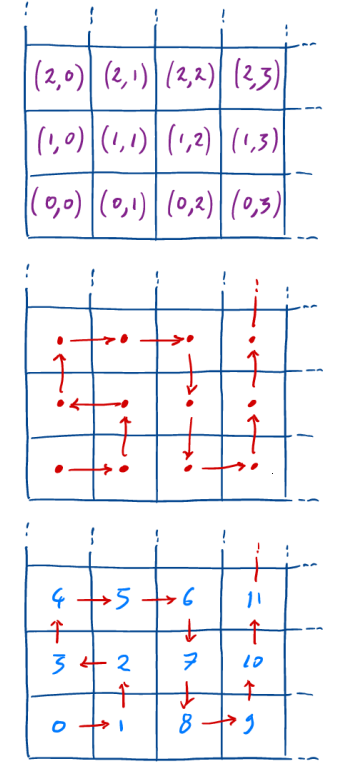
\includegraphics[width=2.82cm]{immagini/aleph2.png}
\end{wrapfigure}
Ci sono diverse vie per illustrare questo risultato. Per esempio, possiamo rappresentare le coppie $(x,y) \in \omega \times \omega$ sotto la specie di una griglia a maglie quadrate.
Poi disegnare un percorso che pare visitare tutte le maglie della griglia, con sufficiente apparenza di regolarità, possibilmente, da convincere il lettore che vi debba essere un metodo.
Infine numeriamo le maglie secondo l'ordine in cui sono visitate dal percorso. Avremo così numerato tutte le coppie di numeri naturali del disegno.\\
Altrimenti, è possiamo esibire delle bigezioni esplicite, per esempio:
\[ f(x,y) = 2^x \cdot (2y + 1) - 1 \qquad g(x,y) = \frac{(x+y)^2 + 3x + y}{2}
	\]
È possibile anche scrivere i due numeri della coppia in base 10 a cifre alternate, tipo: $(\textcolor{blue}{64},\textcolor{red}{4096}) \mapsto \textcolor{red}{4}\textcolor{cyan}{0}\textcolor{red}{0}\textcolor{red}{9}\textcolor{cyan}{0}\textcolor{blue}{6}\textcolor{red}{6}\textcolor{red}{4}\textcolor{blue}{4}$.\\

\newpage
\hspace{-0.43cm}\emph{Dimostrazione.}\hspace{-0.20cm} Innanzitutto definiamo su $\omega \times \omega$ un ordinamento come segue:
	\begin{wrapfigure}[9]{l}{2.5cm}
		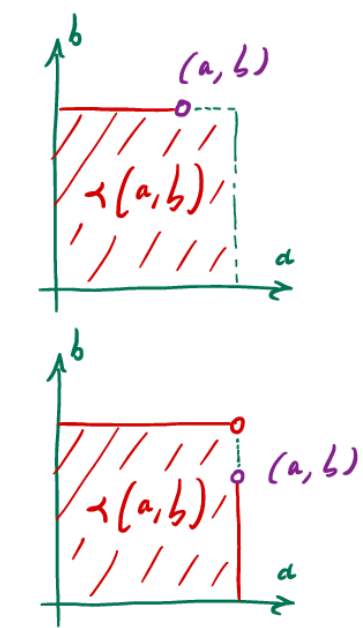
\includegraphics[width=2.5cm]{immagini/ordine_omega.png}
	\end{wrapfigure}
	\[ \begin{split}
		(a,b) \prec (a',b') &\Mydef \max(a,b) < \max(a',b') \\
							&\lor (\max(a,b) = \max(a',b') \land a < a') \\
							&\lor (\max(a,b) = \max(a',b') \land a = a' \land b < b')
	\end{split}
		\]
	ossia per confrontare $(a,b)$ con $(a',b')$, si confrontano prima $\max(a,b)$ e $\max(a',b')$; a parità si confrontano $a$ ed $a'$; se queste coincidono, allora si confrontano $b$ e $b'$.
	\textcolor{MidnightBlue}{L'idea è che le coppie $\prec$ di una certa $(a,b)$ fissata sono tutte contenute nel quadrato $\{0,\ldots,\max(a,b)\} \times \{0,\ldots,\max(a,b)\}$, per cui sono in numero finito, e quindi si ha $(\omega \times \omega, \prec)$ isomorfo a $(\omega,<)$.}\\
	Formalmente, iniziamo col verificare che $\prec$ sia effettivamente un ordine stretto e totale.
	\begin{itemize}
		\item \underline{irriflessività}: immediata dal fatto che confrontare $(a,b)$ con se stessa da un OR con tre alternative tutte necessariamente false a causa dell'irriflessività di $<$.
		\item \underline{transitività}: data $(a,b) \prec (a',b) \prec (a'',b'')$ vogliamo ottenere che $(a,b) \prec (a'',b'')$. Dalle disuguaglianze precedenti segue $\max(a,b) \leq \max(a',b') \leq \max(a'',b'')$, se una di queste disuguaglianze è stretta allora $(a,b) \prec (a'',b'')$ e si conclude,
		altrimenti $\max(a,b) = \max(a',b') = \max(a'',b'')$, e segue dalla definizione di $\prec$ che $a \leq a' \leq a''$. Nuovamente, se una delle disuguaglianze è strette abbiamo concluso, altrimenti per definizione abbiamo $b \leq b' \leq b''$, e necessariamente una delle disuguaglianze deve essere stretta,
		altrimenti all'inizio avremmo avuto un'uguaglianza, che è assurdo, per cui si conclude necessariamente.
		\item \underline{totalità}: basta osservare che se per $(a,b)$ ed $(a',b')$ non vale nessuna delle due fra $\prec$ e $\succ$, allora necessariamente $a = a'$ e $b = b'$, che rende anche in questo caso vera la definizione di ordinamento totale.
	\end{itemize}
	Ora vogliamo dire che $(\omega \times \omega, \prec) \sim (\omega, <)$, in tal modo, avendo un'isomorfismo di ordini, avremmo in particolare una bigezione tra $\omega$ e $\omega \times \omega$.
	Partiamo dall'osservazione che se $(a,b) \in \omega \times \omega$ allora possiamo definire:
	\[ (\omega \times \omega)_{(a,b)} \Mydef \{(x,y) \in \omega \times \omega | (x,y) \prec (a,b)\}
		\]
	detto il ``\vocab{segmento iniziale} determinato da $(a,b)$ su $(\omega \times \omega,\prec)$''. Tale segmento iniziale è finito, infatti $(\omega \times \omega)_{(a,b)} \subseteq s(\max(a,b)) \times s(\max(a,b))$, dove il RHS è un insieme finito e quindi tutti i suoi sottoinsiemi sono finiti.\\
	Ci serve dire: \textcolor{red}{1.} $(\omega \times \omega, \prec)$ è bene ordinato \textcolor{red}{2.} $(\omega \times \omega, \prec)$ è illimitato \textcolor{red}{3.} ogni sottoinsieme non vuoto e superiormente limitato di $\omega \times \omega$ ha un massimo.
	\begin{enumerate}[1.]
		\item Dato $A \subseteq \omega \times \omega$ con $A \ne \emptyset$, possiamo fissare $a \in A$ e considerare $(\omega \times \omega)_a \cap A$. Se tale intersezione è vuota allora si vede banalmente che $a$ è il minimo di $A$. Se l'intersezione è non vuota, allora è un sottoinsieme di un insieme finito e totalmente ordinato, dunque ha minimo $m \in A$ e tale minimo 
		lo è proprio per tutti gli elementi di $A$, infatti, preso $x \in A \setminus((\omega \times \omega)_a \cap A)$, si ha $m < a \leq x$.
		\item Dato $(a,b) \in \omega \times \omega$, $(a,b) \prec (s(a),s(b))$, dunque $\omega \times \omega$ è illimitato.
		\item Dato $A \subseteq \omega \times \omega$ non vuoto e superiormente limitato da $(a,b) \in \omega \times \omega$, abbiamo che $A \subseteq (\omega \times \omega)_{(a+1,b+1)}$, dunque è finito, e quindi ammette massimo perché $\prec$ è totale e valgono le osservazioni fatta in precedenza.
	\end{enumerate}
$\hfill\square$

\subsection{Numeri interi e razionali}
Usando la proposizione appena dimostrata, potremmo dimostrare, per esempio, che $\ZZ$ e $\QQ$ sono numerabili, se non fosse che non abbiamo ancora definito questi oggetti. Allo scopo, ricordiamo che - \hyperref[3.73]{esercizio} - una relazione di equivalenza
induce un insieme di classi di equivalenza.

\begin{definition}[$\ZZ$]
	Definiamo $\ZZ$ come l'insieme delle classi di equivalenza su $\omega \times \omega$ indotte dalla relazione:
	\[ (a,b) \sim_\ZZ (a',b') \Mydef a + b' = b + a' \, \footnote{Moralmente: ``$(a,b) = a - b$''.}
		\]
\end{definition}

\begin{exercise}
	Dimostrare che $\sim_\ZZ$ è una relazione di equivalenza.
\end{exercise}

\begin{example}[Operazioni su $\ZZ$]
	Definiamo $+,-,\cdot$ su $\ZZ$ mediante:
	\begin{align*}
		[(a,b)]_\ZZ + [(a',b')]_\ZZ &\Mydef [(a+a',b+b')]_\ZZ \\
		-[(a,b)]_\ZZ &\Mydef [(b,a)]_\ZZ \\
		[(a,b)]_\ZZ \cdot [(a',b')]_\ZZ &\Mydef [(a\cdot a' + b \cdot b', a \cdot b' + a' \cdot b)]_{\ZZ}
	\end{align*}
	dimostra che $\ZZ$, con queste operazioni, è un anello commutativo con identità: $1 \Mydef [(1,0)]_\ZZ$. 
\end{example}

\begin{definition}[$\QQ$]
	Definiamo $\QQ$ come l'insieme delle classi di equivalenza su $\ZZ \times (\omega\setminus\{0\})$ indotte dalla relazione:
	\[ (n,d) \sim_\QQ (n',d') \Mydef n \cdot d' = n' \cdot d \, \footnote{Moralmente: ``$(n,d) = \frac nd$''.}
		\]
\end{definition}

\begin{exercise}
	Dimostrare che $\sim_\QQ$ è una relazione di equivalenza.
\end{exercise}

\begin{exercise}[Operazioni su $\QQ$]
	Definisci $+,-,\cdot$ e $\square^{-1}$ su $\QQ$ nella maniera ragionevole e dimostra che $\QQ$ è un campo.
\end{exercise}

\begin{exercise}[Ordinamento su $\QQ$]
	Definisci la relazione $<$ su $\QQ \times \QQ$ dicendo che $q \in \QQ$ è positivo se $q = [(n,d)]_\QQ$, con $n,d \in \omega\setminus\{0\}$, e dicendo che $a < b$ se e solo se $b - a$ è positivo.
	Dimostra che questo è un ordine totale e \vocab{denso}, cioè:
	\[ \forall a,b \in \QQ \; a < b \rightarrow \exists c \in \QQ \; a< c <b \, \footnote{Typo di Mamino.}
		\]
\end{exercise}

\begin{note}
	Gli esercizi precedenti sono tediosi, ma non sono difficili. Nel resto del corso daremo per scontate le proprietà aritmetiche elementari di $\ZZ$ e $\QQ$.
	D'ora innanzi scriveremo:
	\[ a - b \Mydef [(a,b)]_{\ZZ} \qquad \frac{n}{d} \Mydef [(n,d)]_\QQ
		\]
\end{note}

Per dimostrare la numerabilità di $\ZZ$ e $\QQ$, è comodo richiamare ancora un \hyperref[disuguaglianze_senza_AC2]{esercizio}, però, questa volta, lo risolviamo\footnote{La soluzione riportata all'esercizio di riferimento è quella di Mamino.}.

\begin{corollary}[Caratterizzazione della al più numerabilità]
	\label{disugcardnum}
	Un insieme $A \ne \emptyset$ è al più numerabile se e solo se esiste $f : \omega \rightarrow A$ surgettiva.\footnote{D'ora in avanti le disuguaglianze che danno al più numerabile ottenute mediante mappe surgettive saranno quindi legittime.}
\end{corollary}

\begin{proof}
	La freccia $\Longleftarrow$ deriva dall'esercizio citato prima. Per l'inverso, supponiamo $A$ al più numerabile e mostriamo che c'è sempre una mappa surgettiva tra $\omega$ ed $A$.
	Per ipotesi esiste $g : A \hookrightarrow \omega$ - iniettiva -, essendo $A \ne \emptyset$ possiamo fissare $a \in A$ e definire la seguente mappa:
	\[ f : \omega \to A : x \mapsto \begin{cases}
										g^{-1}(x) &\text{se $x \in \Imm(g)$} \\
										a &\text{altrimenti}
									\end{cases}
		\]
	tale mappa è naturalmente ben definita ed è surgettiva in quanto stiamo semplicemente estendendo la mappa bigettiva $g^{-1} : \omega\supseteq\Imm(g) \to A$.
\end{proof}

\begin{notation}[Successione - enumerazione]
	Con \vocab{successione} (numerabile) intendiamo semplicemente una funzione con dominio $\omega$, per cui:
	\[ \alpha = \{\alpha_i\}_{i \in \omega} \Mydef \alpha : \omega \to \ldots: i \mapsto \alpha_i
		\]
	cioè $\alpha$ è un ``elenco numerabile'' - non necessariamente esaustivo - degli elementi dell'insieme di arrivo. Per \vocab{enumerazione}
	intendiamo una successione (numerabile) surgettiva, tale per cui, detto $A$ l'insieme di arrivo, si ha $\Imm(\alpha) = A$, o - informalmente - $A = \{\alpha_i | i \in \omega\}$.
\end{notation}

\textcolor{MidnightBlue}{Il corollario sopra, quindi, non ci dice altro che $A \ne \emptyset$ è al più numerabile se e solo se ha almeno un'enumerazione.}

\begin{example}[L'insieme dei numeri interi è numerabile]
	$\ZZ$ è numerabile.
\end{example}

\begin{proof}
	La funzione $\omega \times \omega \to \ZZ : (a,b) \mapsto a - b$ è surgettiva per definizione (è la proiezione al quoziente di $\omega \times \omega$ modulo $\sim_\ZZ$, che sappiamo essere sempre surgettiva, in questo caso stiamo indicando le classi $[(a,b)]_\ZZ$ con $a - b$, ma sono sempre classi di equivalenza), e $\omega \times \omega$ è numerabile\footnote{$|\omega \times \omega| = \aleph_0 \cdot \aleph_0 = \aleph_0$.} dunque $|\ZZ|\leq \aleph_0$.\\
	D'altro canto, la funzione $\omega \rightarrow \ZZ : n \mapsto [(n,0)]_\ZZ$ è iniettiva, infatti $[(n,0)]_\ZZ = [(m,0)]_\ZZ \iff (n,0) \sim (m,0) \iff n = m$ (per definizione di $\sim_\ZZ$), dunque $\aleph_0 \leq |\ZZ|$, pertanto - per \hyperref[CB]{Cantor-Bernstein} - $|\ZZ| = \aleph_0$.
\end{proof}

\begin{example}[L'insieme dei numeri razionali è numerabile]
	$\QQ$ è numerabile.
\end{example}

\begin{proof}
	Come nell'esempio precedente, la proiezione al quoziente $\ZZ \times (\omega \setminus\{0\}) \rightarrow \QQ : (n,d) \mapsto \frac{n}{d}$ (dove la frazione è un'abbreviazione per la classe di equivalenza $[(n,d)]_\QQ$), è surgettiva per costruzione, inoltre $|\ZZ \times (\omega \setminus\{0\})| = |\ZZ| \cdot |\omega \setminus\{0\}| = \aleph_0 \cdot \aleph_0 = \aleph_0$, dunque vale il 
	\hyperref[disugcardnum]{corollario} sulla disuguaglianza tra cardinalità, pertanto $\aleph_0 \geq |\QQ|$.\\
	Viceversa, la funzione $\omega \rightarrow \QQ : n \mapsto \frac{n}{1}$ è iniettiva, infatti $\frac n1 = \frac m1 \iff n \cdot 1 = m \cdot 1 \iff m = n$, dunque per definizione si ha $\aleph_0 \leq |\QQ|$. Da cui per \hyperref[CB]{Cantor-Bernstein} $|\QQ| = \aleph_0$.
\end{proof}

Adesso, ci piacerebbe poter dire che, se abbiamo un insieme $A$ al più numerabile, e tutti i suoi elementi sono, a loro volta, insiemi al più numerabili, allora
$\bigcup A$ è al più numerabile \textcolor{MidnightBlue}{- ovvero un'unione al più numerabile di insiemi al più numerabili è a sua volta al più numerabile}.\\
D'altro canto è ragionevole: se esiste una enumerazione $\{a_i\}_{i \in \omega}$ di $A$, e, per ogni $i \in \omega$, esiste una enumerazione di $a_i$, cioè esiste:
\[ \alpha_i : \omega \twoheadrightarrow a_i : j \mapsto \alpha_i(j) = \alpha_{i,j}
	\]
tale per cui $a_i = \Imm(\alpha_i) = \{\alpha_{i,j}\}_{j \in \omega}$, allora possiamo mandare surgettivamente - cioè enumerare - $\omega \times \omega$ in $\bigcup A$ mandando ogni coppia $(i,j)$ nel $j$-esimo elemento dell'$i$-esimo elemento di $A$, $(i,j) \mapsto \alpha_{i,j}$,
e, siccome $\omega \times \omega$ numerabile, allora per il \hyperref[disugcardnum]{corollario} $|A| \leq \aleph_0$.\\
L'\textcolor{red}{errore} è credere di poter fissare una enumerazione $\alpha_i$ di $a_i$ per ogni $i \in \omega$. Usando l'assioma della scelta potremo farlo, ma, per ora, non abbiamo modo, in generale, di procurarci la funzione che associa ogni naturale ad una enumerazione dell'elemento di $A$ da lui indicizzato, $i \mapsto \alpha_i$.
Possiamo però assumere di averla, così si corregge il ragionamento impreciso di prima.

\begin{proposition}[$|A| \leq \aleph_0 \implies |\bigcup A| \leq \aleph_0$]
	Sia $A = \{a_i \in A| i \in \omega\}$ e \textcolor{red}{sia $\{\alpha_i\}_{i \in \omega}$ una successione di funzioni}\footnote{Che stiamo appunto assumendo di avere già, altrimenti serve AC.} tali per cui,
	per ogni $i \in \omega$, si ha che $\alpha_i : \omega \twoheadrightarrow a_i$ è una enumerazione di $a_i$, allora $\left|\bigcup A\right| \leq \aleph_0$.
\end{proposition}

\begin{proof}
	Basta osservare che la funzione:
	\[ f : \omega \times \omega \to \bigcup A : (i,j) \mapsto \alpha_i(j) = \alpha_{i,j}
		\]
	è surgettiva e vale quindi il solito \hyperref[disugcardnum]{corollario}. Infatti, dato $a \in \bigcup A$,
	poiché $A = \{a_i\}_{i \in \omega}$, allora $a \in a_i$, per qualche $i \in \omega$, e poiché $a_i = \Imm(\alpha_i)$ - qui stiamo usando che gli elementi di $A$ sono a loro volta al più numerabili -,
 	allora esiste $j \in \omega$ tale per cui $\alpha_i(j) = a$.
\end{proof}

\pagebreak

\begin{notation}
	Data una funzione $f : I \rightarrow S$ definiamo:
	\[ \bigcup_{i \in I} f(i) \Mydef \bigcup f[I]
		\]
	Così, per esempio, se $A = \{a_i | i \in \omega\}$:
	\[ \bigcup A = \bigcup_{i \in \omega} a_i \;\textcolor{MidnightBlue}{= \{x | \exists i \in \omega \; x \in a_i\}}
		\]
\end{notation}

\begin{definition}
	[Parti finite]
	Definiamo le \vocab{parti finite} di un insieme $A$ come:
	\[ \psf(A) \Mydef \{X \in \ps(A) : |X| < \aleph_0\}
		\]
\end{definition}

\begin{proposition}[Insieme al più numerabile $\implies$ parti finite al più numerabile]
	$|A| \leq \aleph_0 \rightarrow |\psf(A)| \leq \aleph_0$.
\end{proposition}

\begin{proof}
	Il caso $A = \emptyset$ è immediato. Assumiamo $A \ne \emptyset$, sia:
	\[ \ps^{\leq n} = \{X \in \ps(A) : |X| \leq n\}
		\]
	siccome $\psf(A) = \bigcup_{n \in \omega} \ps^{\leq n}(A)$, basta esibire una successione di enumerazioni $n \mapsto (\alpha_n \twoheadrightarrow \ps^{\leq n}(A))$, per poter usare il corollario sull'unione - così da evitare AC.\\
	Essendo $|\omega \times A| = \aleph_0$ dall'ipotesi, possiamo fissare  $f : \omega \twoheadrightarrow \omega \times A : x \mapsto (f_1(x),f_2(x))$\footnote{Avendo fissato una $f$ a caso $f_1$ ed $f_2$ sono di fatto funzioni surgettive - entrambe da $\omega$ al rispettivo insieme - a caso.}
	surgettiva (in realtà anche bigettiva). A questo punto possiamo costruire la successione di enumerazioni $(\alpha_n)_{n \in \omega}$ - 
	con $\alpha_n$ enumera $\ps^{\leq n}(A)$ per ogni $n \in \omega$ - per ricorsione numerabile prima forma come segue:
	\begin{itemize}
		\item[$\boxed{m = 0}$] In questo caso $\ps^{=0}(A) = \{\emptyset\}$, dunque $\alpha_0$ è la funzione che mappa tutti i naturali in 0, cioè $\alpha_0 = \{(n,0)\}_{n \in \omega}$.
		\item[$\boxed{m \implies m + 1}$] Data un'enumerazione $\alpha_m$ di $\ps^{\leq m}(A)$, definiamo l'enumerazione $\alpha_{m + 1}$ di $\ps^{\leq m + 1}(A)$ nella maniera seguente:
		\[ 	\alpha_{m + 1} : \omega \rightarrow \ps^{\leq m + 1} : x \mapsto \begin{cases}
			\emptyset &\text{se $x = 0$} \\
			\underbrace{\alpha_m(\overbrace{f_1(x-1)}^{\textcolor{MidnightBlue}{\in \; \omega}})}_{\textcolor{MidnightBlue}{\in \;\ps^{\leq m}(A)}} \cup \{\underbrace{f_2(x - 1)}_{\textcolor{MidnightBlue}{\in A}}\}\;\textcolor{MidnightBlue}{\ne \;\emptyset} &\text{altrimenti}
			\end{cases}
		\]
		\textcolor{MidnightBlue}{di fatto - a parte lasciare un insieme vuoto - stiamo prendendo tutti gli insiemi in $\ps^{\leq m}(A)$ e ci stiamo aggiungendo un elemento di $A$\footnote{Una sorta di shift per la cardinalità.} - va verificato che questa costruzione mantenga la surgettività e lo faremo a breve.}
	\end{itemize}
	Verifichiamo ora per induzione che la successione che abbiamo costruito ricorsivamente $(\alpha_n)_{n \in \omega}$ di enumerazioni dei $\ps^{\leq n}(A)$ sia effettivamente tale, ovvero che $\alpha_n$ sia una mappa surgettiva da $\omega$ in $\ps^{\leq n}(A)$ per ogni $n \in \omega$.
	\begin{itemize}
		\item[$\boxed{m = 0}$] La successione costante $\alpha_0 = \{(n,0)\}_{n \in \omega}$ è banalmente surgettiva.
		\item[$\boxed{m \implies m + 1}$] Per ipotesi induttiva la successione $\alpha_m : \omega \twoheadrightarrow \ps^{\leq m}(A)$ è surgettiva, vogliamo verificare che anche $\alpha_{m + 1} : \omega \to \ps^{\leq m + 1}(A)$ lo è.
		Dato $Y \in \ps^{\leq s(m)}(A)$ si danno due casi. Se $Y = \emptyset$, allora per costruzione $Y = \alpha_{s(m)}(0) = \emptyset$. Altrimenti siamo nel caso in cui esiste almeno un elemento $y \in Y$.\\
		In questo caso necessariamente $|Y\setminus\{y\}| \leq m$, quindi per ipotesi induttiva - cioè $\alpha_m$ surgettiva - $Y \setminus\{y\} = \alpha_m(t)$ per qualche $t \in \omega$.
		Per la surgettività di $f : \omega \twoheadrightarrow \omega \times A$, la coppia $(t,y)$ è immagine di qualche $x \in \omega$, cioè $f(x) = (f_1(x),f_2(x)) = (t,y)$.
		Segue quindi che proprio $x+1$ è una controimmagine di $Y$:
		\begin{align*}
			\alpha_{m + 1}(x+1) &= \alpha_m(f_1(x)) \cup \{f_2(x)\} &&(\text{definizione $\alpha_{m+1}$})\\
							   &= \alpha_m(t) \cup \{y\} &&(f(x) = (t,y)) \\
							   &= (Y \setminus\{y\}) \cup \{y\} = Y &&(\text{Hp. induttiva})
		\end{align*}
	\end{itemize}
\end{proof}

\paragraph*{Applicazione}\mbox{}\\
Dimostriamo che l'insieme dei numeri reali algebrici $\A_{\RR}$\footnote{Sarebbe $\overline{\QQ} \cap \RR$.} è numerabile. Per questa applicazione, assumiamo le proprietà elementari di $\RR$.
L'insieme $\A_{\RR}$ è definito come l'insieme degli $x \in \RR$ che sono zeri di qualche polinomio a coefficienti razionali:
\[ \A_{\RR} \Mydef \{x \in \RR | \exists p(x) \in \QQ[x]\setminus\{0\} \; p(x) = 0\}
	\]
I numeri reali che non sono algebrici si dicono \vocab{trascendenti} (= $\RR\setminus(\overline{\QQ} \cap \RR)$), siccome - formalmente, vedremo questo risultato in seguito - $\RR$ non è numerabile, deduciamo dalla numerabilità di
$\A_{\RR}$ che ci sono numeri reali trascendenti.\\
Dimostriamo, intanto, che l'insieme $\QQ[x]$, dei polinomi a coefficienti razionali nella indeterminata $x$, è numerabile.
Possiamo identificare un polinomio:
\[ p(x) = a_0 + a_1x + a_2x^2 + \ldots + a_d x^d
	\]
con l'insieme dei suoi monomi:
\[ p(x) = \{a_0,a_1x,a_2x^2,\ldots,a_dx^d\}
	\]
e ciascun monomio con la coppia (grado, coefficiente):
\[ p(x) = \{(0,a_0),(1,a_1),\ldots,(d,a_d)\}\,\footnote{Può essere pensata come funzione da $d$ in $\QQ$, o come una funzione da $\omega$ a $\QQ$ a supporto finito.}
	\]
Formalmente, come accade per i numeri, le coppie ordinate, le funzioni, etc., anche i polinomi non sono oggetti atomici della teoria degli insiemi: occorre, in qualche modo, fissare una codifica.
Quella appena descritta è una codifica ragionevole. Rappresentando i polinomi in questo modo:
\[ \QQ[x] \subseteq \psf(\omega \times \QQ) \, \footnote{Più precisamente $\QQ[x] = \bigcup_{n \in \omega} n \times \QQ \subseteq \psf(\omega \times \QQ)$.}
	\]
per cui, essendo che $|\omega \times \QQ| = \aleph_0 \implies |\psf(\omega \times \QQ)| = \aleph_0$, si ha $|\QQ[x]| \leq \aleph_0$.
Inoltre è elementare che $\QQ \hookrightarrow \QQ[x]$ (ad esempio $q \mapsto \{(0,q)\}$ è una mappa iniettiva che dà tutti i polinomi di grado 0), in tal modo si ha anche l'altra disuguaglianza di 
cardinalità e quindi - come al solito per \hyperref[CB]{Cantor-Bernstein} - $|\QQ[x]| = \aleph_0$. Venendo ad $\A_{\RR}$ abbiamo una facile surgezione:
\begin{multline*}
	f : (\QQ[x]\setminus\{0\}) \times \omega \to \A_{\RR} :\\
	 (p,i) \mapsto \text{``la $i$-esima radice di $p$ se questa esiste, altrimenti 0''}
\end{multline*}
Vediamo, però, in maggior dettaglio come si può rappresentare $f$ mediante una formula insiemistica.
\[
	\text{``$\alpha$ è la $i$-esima radice di $p$''} \equiv
	p(\alpha) = 0 \land |\{x \in \RR | x \leq \alpha \land p(x) = 0\}| = |i|
\]
\begin{multline*}
	y = f(p,i) \equiv \text{``$y$ è la $i$-esima radice di $p$''} \\
	\land(y = 0 \land \neg \exists \alpha \in \RR \; \text{``$\alpha$ è la $i$-esima radice di $p$''})
\end{multline*}
Per separazione esiste, quindi, $f$, e, di conseguenza $|\A_{\RR}| \leq \aleph_0$. La disuguaglianza opposta è immediata perché $\QQ \subseteq \A_{\RR}$ - è facile scrivere un polinomio in $\QQ[x]$ che abbia come radice un qualsiasi $q \in \QQ$ fissato.

\begin{exercise}[Ogni gruppo finitamente generato è al più numerabile]
	Dato un insieme $X$, una funzione $f : X \times X \to X$, e un sottoinsieme $A \subseteq X$ al più numerabile, dimostra che esiste un $\ol A \subseteq X$ al più numerabile tale che $A \subseteq \ol A$\footnote{Typo di Mamino, questa ipotesi manca nelle dispense, ma c'è scritta nel 2021.}
	e $f[\ol A \times \ol A] \subseteq \ol A$. Concludi che un gruppo finitamente generato è al più numerabile.
\end{exercise}

\begin{soln}[DA COMPLETARE]
	L'idea per risolvere la prima parte è ottenere $\ol A$ come unione numerabile di una successione che parta da $A$ e che ad ogni passaggio nel faccia l'immagine via $f$, in modo tale che l'unione rispetti poi tutte le proprietà volute.
	Per questa ragione definiamo per ricorsione numerabile prima forma la seguente successione:
	\[ A_n : \omega \to \ps(X) : \begin{cases}
		A_0 = 0 \\
		A_{n + 1} = f[A_n \times A_n] \cup A_n
	\end{cases}
		\]
	e quindi $\ol A := \bigcup_{n \in \omega} A_n$. Naturalmente, essendo $A_n \subseteq X$ per ogni $n \in \omega$ - per definizione di $f$ -, si ha che $\ol A \subseteq X$; inoltre, presi $x,y \in \ol A$ si ha $x \in A_i$ e $y \in A_j$, per $i, j \in \omega$, poiché $A_n \subseteq A_{n + 1}$, cioè la successione è crescente,
	si ha $x,y \in A_{\max(i,j)}$, per cui per definizione di $f$ si conclude $f(x,y) \in A_{\max(i,j) + 1} \subseteq \ol A$.\\
	Ci rimane da verificare che $|\ol A| \leq \aleph_0$, per fare ciò vogliamo usare il corollario dell'unione - che evita AC -, dobbiamo quindi procurarci una 
	successione di enumerazioni $n \mapsto \alpha_n$, con $\alpha_n : \omega \twoheadrightarrow A_n$. Definiamo la successione per ricorsione numerabile.
	\begin{itemize}
		\item[$\boxed{n = 0}$] Per ipotesi $A_0 = A$ è al più numerabile quindi possiamo fissare una sua enumerazione ed usare quella come $\alpha_0$.
		\item[$\boxed{n \implies n + 1}$] Supponiamo di avere per ipotesi induttiva $\alpha_n : \omega \to A_n$ e costruiamo $\alpha_{n + 1} : \omega \to A_{n + 1}$
	\end{itemize}
	Dimostriamo ora per induzione che la successione così definita è effettivamente una successione di enumerazione per gli $A_n$\footnote{Come nella proposizione
	sulle parti finite, non solo la successione di enumerazioni ci permette di applicare il corollario sull'unione, ma ha come conseguenza - cosa che stiamo per dimostrare per induzione - che $\forall n \in \omega \; |A_n| \leq \aleph_0$, che a priori non sapevamo.}.
	\begin{itemize}
		\item[$\boxed{n = 0}$] Abbiamo preso già $\alpha_0$ enumerazione nelle costruzione per ricorsione, quindi non c'è altro da dimostrare.
		\item[$\boxed{n \implies n + 1}$] Supponiamo che $\alpha_n$ sia surgettiva e dimostriamo che lo è $\alpha_{n + 1} : \omega \to A_{n + 1}$. Dato $y \in A_{n + 1} = f[A_n \times A_n] \cup A_n$,
		ci sono tre possibilità:
		\begin{itemize}
			\item se $y \in A_n \setminus f[A_n \times A_n]$: in tal caso, essendo $\alpha_n$ surgettiva esiste $x \in \omega$ tale per cui $\alpha_n(x) = y$
			\item se $y \in A_n \cap f[A_n \times A_n]$: in tal caso $y = f(z)$, con $z = (a,b) \in A_n \times A_n$, e di nuovo, per surgettività di $\alpha_n$ esistono $a',b' \in A_n$, per cui $\alpha_n(a') = a$ e $\alpha_n(b') = b$
			\item se $y \in f[A_n \times A_n] \setminus A_n$:
		\end{itemize}
	\end{itemize}
	Per la seconda parte, dato un gruppo $G$ e $S \subseteq G$, tale che $|S| < \aleph_0$ e $\langle S \rangle = G$, consideriamo la funzione:
	\[ f : G \times G \to G : (x,y) \mapsto xy^{-1}
		\]
	per quanto dimostrato nella prima parte esiste $\overline{S} \subseteq G$ tale che $S \subseteq \ol S$ e $|\ol S| \leq \aleph_0$. Essendo ora $G$ non vuoto e finitamente generato si ha $S \ne \emptyset$,
	per cui $\ol S \ne \emptyset$, verifichiamo dunque che $\ol S$ è un sottogruppo di $G$.
	\begin{itemize}
		\item Essendo $\ol S \ne \emptyset$ esiste $g \in \ol S$, e per ipotesi $e_G = gg^{-1} f(g,g) \in \ol S$.
		\item Dal primo punto segue facilmente che $\forall g \in \ol S \; g^{-1} = e_G \cdot g^{-1} = f(e_G,g) \in \ol S$.
		\item Infine $\forall g,h \in \ol S$, per il punto precedente vale sempre che $h^{-1} \in \ol S$, e per ipotesi $gh = f(g,h^{-1}) \in \ol S$.
	\end{itemize}
	Abbiamo quindi che $\ol S$ è un sottogruppo di $G$ che contiene $S$, per cui è proprio tutto il gruppo, $\ol S = G$, e quindi vale $|G| = |\ol S| \leq \aleph_0$.
\end{soln}

\subsection{Ordini densi numerabili}
Il prossimo risultato che vedremo è, come al solito, dovuto a Cantor, e caratterizza l'ordine di $\QQ$ a meno di isomorfismi.

\begin{definition}[Densità]
	Sia $(A,<)$ totalmente ordinato, e $B \subseteq A$, diciamo che $B$ è \vocab{denso in} $(A,<)$ se:
	\[ \forall x,y \in A \; x < y \rightarrow \exists z \in B \; x < z < y
		\]
	\textcolor{MidnightBlue}{cioè tra due elementi di $A$ c'è sempre un elemento di $B$}.\\
	Inoltre diciamo che $(A, <)$ è \vocab{denso}, cioè è denso in se stesso, se:
	\[ \forall x,y \in A \; x < y \rightarrow \exists z \in A \; x < z < y
		\]
	\textcolor{MidnightBlue}{cioè tra due elementi di $A$ c'è sempre qualche elemento di $A$}.
\end{definition}

\begin{example}[$(\QQ,<)$ è denso in se stesso]
	Abbiamo già osservato, in un esercizio, che $\QQ$ è denso, infatti:
	\[ x < y \rightarrow x < \frac{x+y}{2} < y
		\]
	cioè presi due qualsiasi elementi di $\QQ$, la loro media aritmetica è sempre in mezzo e sta in $\QQ$ (formalmente le due disuguaglianze si giustificano con le operazioni di $\QQ$ + l'ordinamento totale + le proprietà 
	di compatibilità tra operazioni e ordinamento).
\end{example}

\begin{notexample}[$(\omega,<)$ non è denso in se stesso]
	L'insieme $\omega$ con il suo ordinamento naturale non è denso, perché $\not\exists z \in \omega \; 0 < z < 1$.
\end{notexample}

\begin{theorem}[Teorema di isomorfismo di Cantor]
	\label{isoCantor}
	Sia $(A,<)$ un insieme totalmente ordinato tale che:
	\begin{enumerate}[1.]
		\item $|A| = \aleph_0$
		\item $(A,<)$ è denso
		\item $(A,<)$ non ha \vocab{estremi}, ossia non ha né massimo né minimo elemento
	\end{enumerate}
	allora $(A,<)\sim(\QQ,<)$.\footnote{Notare che le proprietà elencate sono cose che abbiamo già verificato che valgono per $\QQ$, quindi questo teorema è la caratterizzazione di $(\QQ,<)$ come ordine totale.}
\end{theorem}

\textcolor{MidnightBlue}{L'idea è di costruire l'isomorfismo per ricorsione. Ad ogni passo della ricorsione avremo $f_i : A_i \rightarrow Q_i$ isomorfismo con $A_i \subseteq A$ finito 
e $Q_i \subseteq \QQ$. Dovremo quindi estendere $f_i$ ingrandendo il suo dominio.
Supponiamo, per esempio, di voler definire $f_{i+1}(x)$ con $x \not \in A_i$. Allora, siccome $A_i$ è finito, per sapere la posizione di $x$ a ciascuno degli elemento di $A_i$, ci basta sapere quale sia l'ultimo elemento prima di $x$,
e quale sia il primo dopo $x$ - diciamo che, per esempio, sono $a_2$  e $a_3$ rispettivamente. Dovremo allora mandare $x$ in un $f_{i+1}(x)$ con $f_i(a_2) < f_{i+1}(x) < f_i(a_3)$, e questo esiste per la densità di $\QQ$.}

\begin{figure}[H]
	\centering
	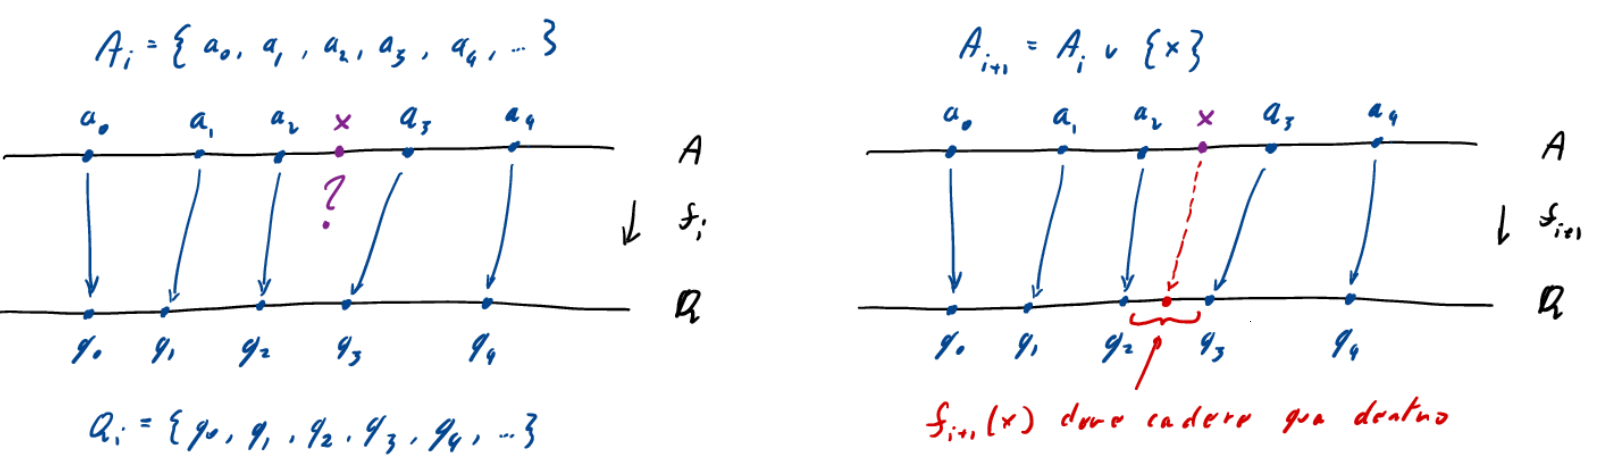
\includegraphics[width = 12cm]{immagini/IsoCantor.png}
\end{figure}

\textcolor{MidnightBlue}{Ragionando simmetricamente, possiamo anche estendere $f_i$, dato un $y \in \QQ$ con $y \not\in Q_i$, in modo tale che $y \in \Imm(f_{i+1})$.}

\begin{figure}[H]
	\centering
	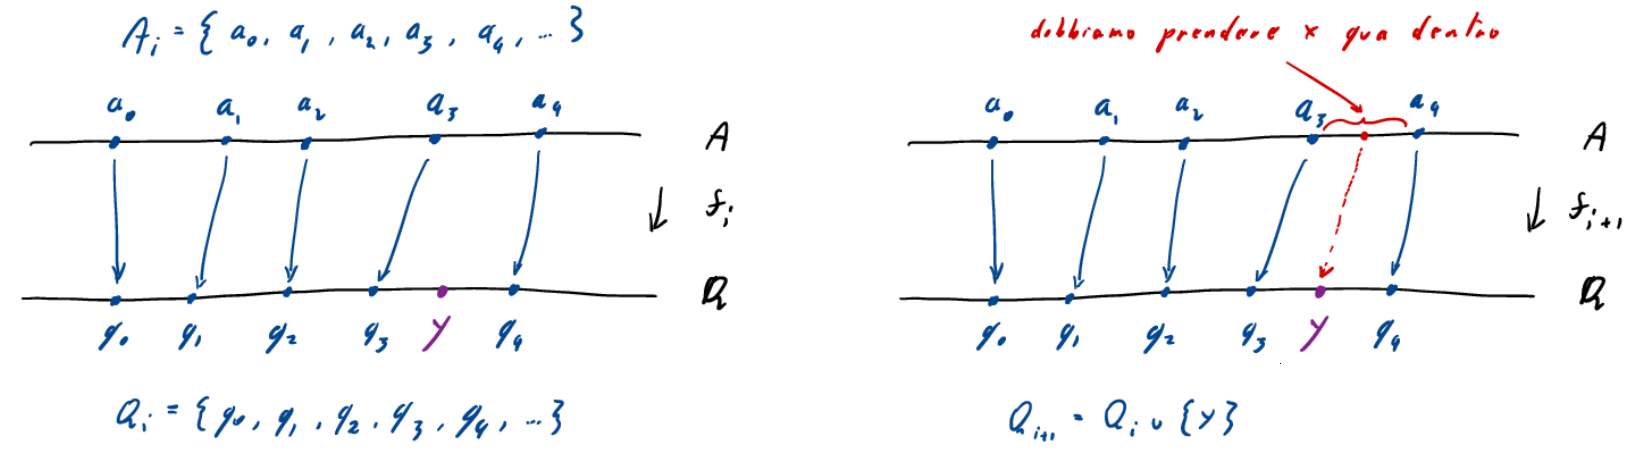
\includegraphics[width = 12cm]{immagini/IsoCantor2.png}
\end{figure}

\textcolor{MidnightBlue}{In definitiva, ci basta quindi fissare un'enumerazione di $A$ e una di $\QQ$, e fare questi passi di estensione in maniera alternata, assicurandoci così di aggiungere al dominio della $f$, uno per uno,
tutti gli elementi di $A$, e di aggiungere all'immagine, uno per uno, tutti gli elementi di $\QQ$. Ci farà comodo la segue osservazione.}

\begin{remark}[L'unione di un insieme di funzioni compatibili è una funzione]
	Sia $F \subseteq \ps(A \times B)$ un insieme di funzioni. Se vale che:	
	\[ \forall f_1,f_2 \in F \; f_{1|\Dom(f_1) \cap \Dom(f_2)} = f_{2|\Dom(f_1) \cap \Dom(f_2)}
			\]
	cioè se le funzioni da $A$ a $B$ coincidono sull'intersezione dei domini a due a due, $\forall x \in \Dom(f_1) \cap Dom(f_2) \; f_1(x) = f_2(x)$, allora $\bigcup F$ è ancora una funzione dall'unione dei domini a $B$:
	\[ \bigcup F : \bigcup\{\Dom(f) | f\in F\} \rightarrow B
		\]
\end{remark}

\begin{proof}
	Bisogna verificare che vale la proprietà fondamentale delle funzioni, ovvero che, se $(x,y_1) \in \bigcup F$ e $(x,y_2) \in \bigcup F$, allora $y_1 = y_2$.\\
	Dalla prima cosa abbiamo che esiste $f_1 \in \bigcup F$ tale che $f_1(x) = y_1$ e, dalla seconda, sappiamo che esiste $f_2 \in \bigcup F$ tale che $f_2(x) = y_2$, ma questo significa - per definizione di dominio -
	che $x \in \Dom(f_1) \cap \Dom(f_2)$, dunque dall'ipotesi si ha che:
	\[ y_1 = f_1(x) \overset{\text{Hp.}}{=} f_2(x) = y_2
		\]
\end{proof}

Siamo ora pronti per dimostrare formalmente il teorema.

\begin{proof}
	Per l'ipotesi 1 possiamo fissare un'enumerazione di $A$ e $\QQ$ rispettivamente:
	\[ A = \{a_i | i \in \omega\} \qquad \QQ = \{q_i | i \in \omega\}
		\]
	vogliamo costruire una successione di funzioni $(f_i)_{i \in \omega}$ tale per cui, per ogni $i \in \omega$:
	\begin{enumerate}[(1)]
		\item $f_i : A_i \rightarrow Q_i$ con $|A_i| = |Q_i| < \aleph_0$.
		\item $f_i$ è un isomorfismo di ordini fra $A_i$ e $Q_i$.
		\item $f_{i} \subseteq f_{s(i)}$ \textcolor{MidnightBlue}{- ossia $f_{s(i)}$ estende $f_i$}.
		\item $\forall j < i \; a_j \in A_i \land q_j \in Q_i$, \textcolor{MidnightBlue}{ossia il dominio e l'immagine contengono sempre almeno i primi $i$ elementi delle rispettive enumerazioni (poi possono contenere anche altro come vedremo dopo nella costruzione):
		\[ 	\{a_0,\ldots,a_{i-1}\} \subseteq \Dom(f_i) = A_i \qquad Q_i = \{q_0,\ldots,q_{i-1}\} \subseteq \Imm(f_i) = Q_i
			\]}
	\end{enumerate}
	Dando per buona l'esistenza e l'unicità della successione sopra, possiamo definire:
	\[ f := \bigcup_{i \in \omega} f_i
		\]
	\begin{itemize}
		\item[$\diamondsuit$] \underline{$f$ è una funzione}: da $(3)$ segue, facilmente per induzione, che $\forall i < j \; f_i \subseteq f_j$, quindi è una successione di funzioni ciascuna che estende la precedente, per cui sono compatibili e l'unione è ancora una funzione.
		\item[$\diamondsuit$] \underline{$f : A \to \QQ = \Imm(f)$}: da $(4)$ vale che $\Dom(f) = \bigcup_{i \in \omega}\Dom(f_i) = \bigcup_{i \in \omega} A_i = A$ e $\Imm(f) = \bigcup_{i \in \omega}\Imm(f_i) = \bigcup_{i \in \omega} Q_i = \QQ$ - dove abbiamo appunto usato
		che dominio e immagine $i$-esimi, $A_i$ e $Q_i$, per (4) contengono i primi $i$-termini della enumerazione. Poiché abbiamo preso come codominio proprio l'immagine $f$ è automaticamente surgettiva. 
		\item[$\diamondsuit$] \underline{$f$ strettamente crescente}: dati $x, y \in A$ tali per cui $x < y$, si ha che $x \in A_i$ e $y \in A_j$, per $i,j \in \omega$, ora detta $t:= \max(i,j)$ si ha che $x,y \in A_t$ e, per $(4)$, $A_t \subseteq f(t)$, con $f_t$ isomorfismo - per (2), segue quindi:
		\[ x < y \leftrightarrow f(x) = f_t(x) < f_t(y) = f(y)
			\]
	\end{itemize}
	Non ci resta altro da fare che costruire la successione $(f_i)_{i \in \omega}$ per ricorsione numerabile - prima forma. Poniamo $f_0 = \emptyset$,
	per costruire $f_{s(i)}$ definiamo prima un passo intermedio $f_{i+0.5}$ \textcolor{MidnightBlue}{- nel primo passo, $f_{i + 0.5}$, estendiamo la funzione aggiungendo $a_{i}$ al dominio (se non ci fosse già), nel secondo passo, $f_{i + 1}$, analogamente, aggiungiamo $q_i$ all'immagine (se non ci fosse già).}
	Data quindi $f_i : A_i \to Q_i$, distinguiamo due casi:
	\begin{itemize}
		\item \underline{se $a_i \in \Dom(f_i)$}: allora $f_{i + 0.5} = f_i$.
		\item \underline{altrimenti}: detto $\overline{j} := \min\{j \in \omega | f_i \cup \{(a_i,q_j)\} \; \text{è un isomorfismo}\}$ \textcolor{MidnightBlue}{(tecnicamente basta strettamente crescente visto che l'immagine è il codominio)},
		poniamo $f_{i + 0.5} = f_i \cup \{(a_i,q_{\ol j})\}$.
	\end{itemize}
	Ora possiamo fare il secondo passo di estensione e definire $f_{i+1}$:
	\begin{itemize}
		\item \underline{se $q_i \in \Imm(f_{i + 0.5})$}: allora $f_{i + 1} = f_{i + 0.5}$.
		\item \underline{altrimenti}: detto $\ol \iota := \min\{\iota \in \omega | f_{i + 0.5} \cup (a_{\ol \iota},q_i) \; \text{è un isomorfismo}\}$ \textcolor{MidnightBlue}{(come prima basta strettamente crescente)}.\footnote{Notare che la costruzione sarebbe stata simmetrica e funzionante nel caso avessimo voluto costruire $f : \QQ \to A$.}
	\end{itemize}
	Le proprietà (1),\ldots,(4) seguono in maniera immediata per induzione, a patto che la costruzione sia ben posta, ossia i minimi esistano. 
	Ad essere precisi, occorre quindi dimostrare, per induzione su $i$, la seguente proposizione:
	\[ \forall i \in \omega \; \text{``la costruzione di $f_i$ è ben posta e valgono (1),\ldots,(4)''}
		\]
	Naturalmente il nel caso $f_0 = \emptyset$ la proposizione è vera a vuoto, vediamo il passo induttivo, ma solo per la buona definizione.\\
	Per verificare che la definizione di $f_{i + 1}$ sia ben posta, supponendo per ipotesi induttiva che $f_i$ lo sia e che valgano per lei le proprietà $(1),\ldots,(4)$,
	bisogna verificare dunque che i minimi esistano in entrambi i passaggi di estensione, e qui entrano in gioco le ipotesi 2 e 3 del teorema. Vediamo che esiste il minimo
	nel primo passaggio di estensione (sarà analogo verificarlo nel secondo). Consideriamo:
	\[ \ol j = \min\{j \in \omega | f_i \cup \{(a_i,q_j)\}\,\text{è un isomorfismo}\}
		\]
	Per ipotesi induttiva, vale $(1)$ per $f_i$, per cui $A_i$ è finito. Detto $n = |A_i|$ (avendo già fatto il caso $i = 0$ sappiamo che $i > 0$ e dalla costruzione $|i| \leq |A_i|$),
	sfruttando il fatto visto che un ordine totale finito è isomorfismo ad un numero naturale possiamo bene ordinare $A_i$ nella maniera seguente:
	\[ A_i = \{\alpha_0,\ldots,\alpha_{n-1}\} \qquad\text{con $\alpha_0<\ldots<\alpha_{n-1}$}
		\]
	Ora, siamo naturalmente nel caso in cui $a_i \not \in \Dom(f_i)$, quindi o $a_i <\alpha_0$, o $\alpha_k < a_i < \alpha_{k+1}$ per
	qualche $k$, o $a_{n-1}<a_i$. Nel primo e terzo caso, rispettivamente, siccome $\QQ$ non ha estremi, c'è un $q_j < f_i(\alpha_0)$, o $q_j > f_i(\alpha_n)$, per cui $f_{i + 0.5} \cup \{(a_i,q_j)\}$ è un isomorfismo.
	Nel secondo caso, per la densità di $\QQ$, esiste $q_j$ con $f_i(\alpha_k)<q_j<f_i(\alpha_{k+1})$ e quindi di nuovo $f_{i + 0.5}  \cup \{(a_i,q_j)\}$ è un isomorfismo. Nella verifica del secondo passo dell'estensione
	faremo lo stesso identico ragionamento con $Q_i$ usando questa volta densità ed illimitatezza di $A$, per trovare gli elementi.
\end{proof}

\begin{corollary}[Ogni ordine al più numerabile è isomorfo ad un sottoinsieme di $\QQ$]
	Sia $(A,<)$ un ordine totale con $|A| \leq \aleph_0$. Allora esiste $B \subseteq \QQ$ tale che $(A,<) \sim (B,<)$ con l'ordinamento indotto su $B$ da $\QQ$.
\end{corollary}

\begin{note}
	Volendo, si potrebbe dimostrare questo corollario ripetendo, con qualche variazione, la dimostrazione del teorema. Ora daremo, però,
	un argomento che, invece, applica il teorema. È comodo definire, prima, il prodotto di ordini.
\end{note}

\begin{definition}[Prodotto lessicografico di ordini]
	Dati $(A,<_A)$ e $(B,<_B)$ definiamo il \vocab{prodotto lessicografico} di ordini come:
	\[ (A,<_A) \times (B,<_B) \Mydef (A \times B, <_{A \times B})
 		\]
	dove $(a,b) <_{A \times B} (a',b') \Mydef (b <_B b') \lor (b = b' \land a <_A a')$.
\end{definition}

\textcolor{MidnightBlue}{Ossia $(A,<_A) \times (B,<_B)$ è il prodotto cartesiano $A \times B$ munito dell'ordine che confronta prima la seconda componente.}\\
Visualmente, si può immaginare il prodotto lessicografico $(A,<_A) \times (B,<_B)$ come ``$(A,<_A)$ ripetuto $(B,<_B)$ volte''.

\begin{figure}[H]
	\centering
	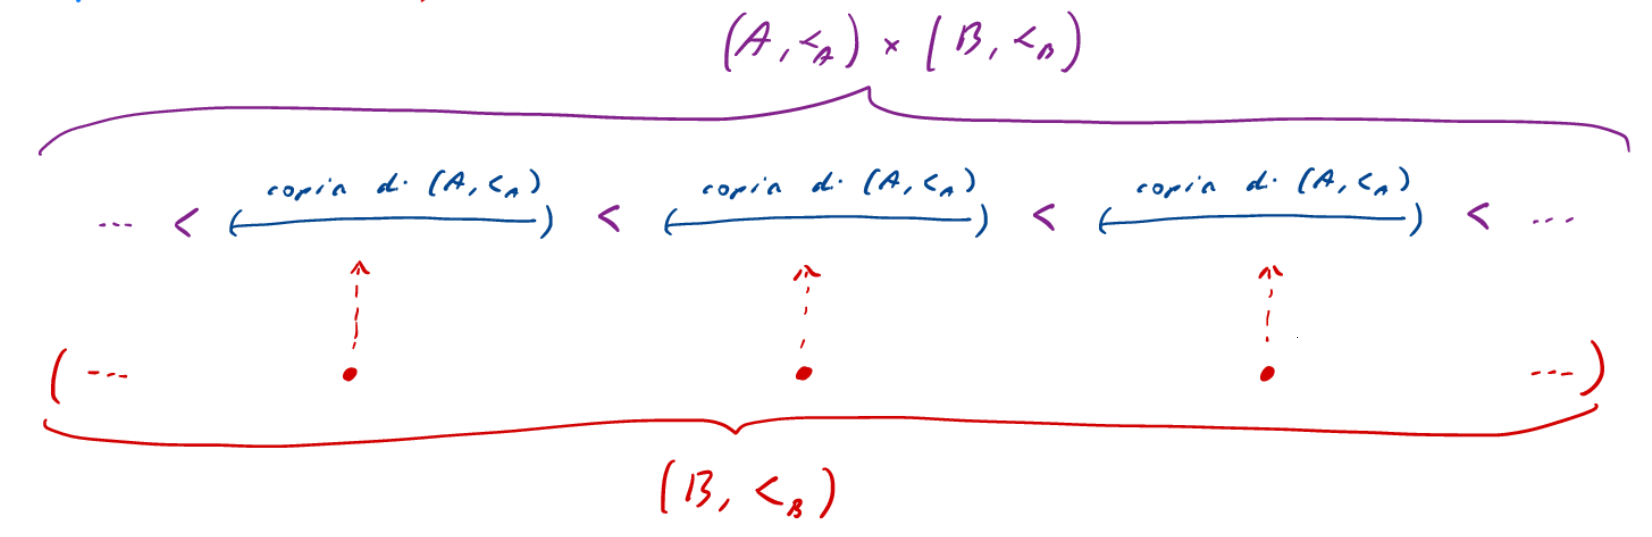
\includegraphics[width = 10cm]{immagini/ordine_lessicografico.png}
\end{figure}

\begin{remark}[Il prodotto lessicografico grafico di ordini totali è un ordine totale]
	Se $(A, <_A)$ e $(B,<_B)$ sono ordini totali, allora anche $(A,<_A) \times (B,<_B)$ lo è.\footnote{È una facile verifica che usa appunto la totalità di $<_A$ e $<_B$.}
\end{remark}

\begin{exercise}[Associatività del prodotto lessicografico]
	Dati $(A,<_A),(B,<_B)$ e $(C,<_C)$ dimostra che:
	\[ ((A,<_A) \times (B,<_B)) \times (C,<_C) \sim (A,<_A) \times ((B,<_B) \times (C,<_C))
		\]
	ossia che il prodotto lessicografico di ordini è associativo a meno di isomorfismi.
\end{exercise}

Veniamo ora alla dimostrazione del corollario

\begin{proof}
	Se $A = \emptyset$ è banale, supponiamo quindi $A \ne \emptyset$ e consideriamo:
	\[ (S,<) \Mydef (\QQ,<) \times (A,<)
		\]
	\begin{figure}[H]
		\centering
		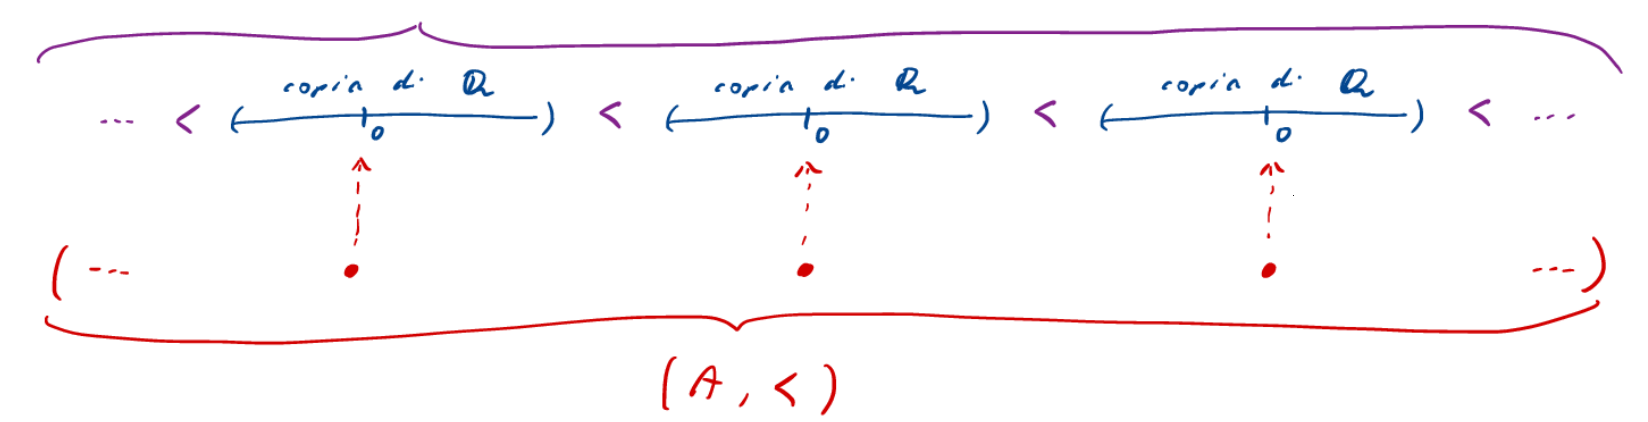
\includegraphics[width = 10cm]{immagini/coroll_iso_cantor.png}
	\end{figure}
	L'insieme $S = \QQ \times A$ è numerabile, inoltre, dato $(q,a) \in \QQ \times A$ abbiamo:
	\[ (q-1,a) < (q,a) < (q+1,a) 
		\]
	quindi $\QQ \times A$ non ha estremi - né superiori né inferiori. Per verificare che è denso, consideriamo $(q_1,a_1) < (q_2, a_2)$ e verifichiamo che in ogni caso c'è sempre un altro elemento di $S$ strettamente nel mezzo.
	\begin{itemize}
		\item Se $a_1 < a_2$, allora $(q_1,a_1) < (q_1+1,a_1) < (q_2,a_2)$ - e funziona per la definizione di ordinamento nel prodotto lessicografico.
		\item Se $a_1 = a_2$ - per cui siamo nella stessa copia di $\QQ$ -, si ha che $(q_1,a_1) < \left(\frac{q_1+q_2}{2},a_1\right) < (q_2,a_2) = (q_2,a_1)$.
	\end{itemize}
	quindi $(S,<)$ è denso e per il \hyperref[isoCantor]{teorema di isomorfismo di Cantor} si ha $(S,<) \sim (\QQ,<)$.
	Infine $A \hookrightarrow \QQ \times A : a \mapsto (0,a)$, quindi, componendo l'immersione (strettamente crescente) con l'isomorfismo trovato, abbiamo che $(A,<)$ è isomorfo ad un sottoinsieme di $(\QQ,<)$. 
\end{proof}

\begin{exercise}[Isomorfismo di Cantor senza l'ipotesi di illimitatezza]
	Dimostra che se $(A,<)$ è denso \textcolor{red}{(ma non necessariamente senza estremi)} e $2 \leq |A| \leq \aleph_0$, allora $(A,<)$ è isomorfismo a uno dei seguenti intervalli di $\QQ$:
	\[ [0,1]_{\QQ} \qquad ]0,1]_{\QQ} \qquad [0,1[_{\QQ} \qquad ]0,1[_{\QQ}
		\]
\end{exercise}

\begin{soln}
	Osserviamo che per l'ipotesi di densità $2 \leq |A| \leq \aleph_0 \implies |A| = \aleph_0$\footnote{Stiamo escludendo l'insieme denso con un solo elemento grazie all'ipotesi che $|A| \geq 2$.}. A questo punto, se $A$ è senza estremi si ha:
	\[ (A,<) \sim (\QQ,<) \sim ]0,1[_\QQ
		\]
	($]0,1[_\QQ$ è totalmente ordinato [ereditariamente dall'ordine di $\QQ$], senza estremi, numerabile [sottoinsieme di $\QQ$ e c'è la mappa $n \mapsto \frac 1n$] e denso [basta prendere la media di due elementi e osservare che sta sempre in mezzo per le proprietà algebriche di $\QQ$]).\\
	Negli altri casi si osserva che:
	\[ [0,1]_{\QQ} = ]0,1[_{\QQ} \,\cup\, \{0,1\}  \qquad ]0,1]_{\QQ} = ]0,1[_{\QQ} \,\cup\, \{1\} \qquad [0,1[_{\QQ} = ]0,1[_{\QQ} \,\cup\, \{0\}
		\]
	vediamo, ad esempio, nel caso di $A$ con entrambi gli estremi, che, detti questi $a$ e $b$, si ha:
	\[ (A\setminus\{a,b\},<_{|A\setminus\{a,b\}}) \sim (\QQ,<) \sim (]0,1[_{\QQ},<)
		\]
	e analogamente negli altri due casi. Fissiamo un isomorfismo $f$ tra $A \setminus \{a,b\}$ e $]0,1[_\QQ$ ed estendiamolo all'isomorfismo voluto:
	\[ f' : A \to [0,1]_\QQ : x \mapsto \begin{cases}
		0 &\text{se $x = a$} \\
		1 &\text{se $x = b$} \\
		f(x) &\text{altrimenti}
	\end{cases}
		\]
	si verifica facilmente che è effettivamente un isomorfismo e negli altri casi si procede in maniera analoga.
\end{soln}

\subsection{Il grafo random}

La tecnica di estendere indefinitamente isomorfismi parziali che ci ha permesso di dimostrare il teorema di isomorfismo di Cantor
si chiama \vocab{back-and-forth}, ed è un metodo fondamentale per trovare isomorfismi fra strutture.\\
Cogliamo questa occasione per suggerire un esercizio di applicazione della medesima tecnica che è un po' complicato. Si tratta di definire il \vocab{grafo random}
o \vocab{grafo di Rado}.

\begin{definition}[Grafo]
	Un \vocab{grafo} $(V,e)$ sull'insieme di vertici $V$ è dato da una relazione $e$ simmetrica \textcolor{MidnightBlue}{($\forall x,y \in V \; (x,y) \in e \leftrightarrow (y,x) \in e$)} e 
	irriflessiva \textcolor{MidnightBlue}{($\forall x \in V \; (x,x) \not\in e$)}.
\end{definition}

\textcolor{MidnightBlue}{L'idea è che $V$ può essere immaginato come un insieme di punti che possono essere connessi da archi. Dire che c'è un arco fra $x$ e $y$ equivale a $(x,y) \in e$.\\}
\mbox{}\\
Partiamo da un'idea intuitiva -  chi ha già seguito un corso di probabilità saprà formalizzare questa cosa in termini precisi. Data una probabilità $p \in \, ]0,1[$ costruiamo un grafo
$G_p$ con insieme di vertici $\omega$ come segue. Per ogni coppia $(i,j) \in \omega \times \omega$ con $i < j$ \textcolor{MidnightBlue}{- cioè la seconda componente è sempre strettamente più grande della prima -}
lanciamo una moneta \textbf{che fa testa con probabilità $p$} - tutte queste monete indipendentemente - e, se viene testa, mettiamo un arco fra $i$ e $j$.\\
Potremmo pensare che i grafi $G_{0.01}$ e $G_{0.99}$ debbano venire molto diversi: uno ha l'1\% degli archi possibili, l'altro ha il 99\%, insomma uno è quasi vuoto, l'altro quasi completo. \textbf{Avviene,
tuttavia, che, con probabilità 1, questi grafi sono isomorfismi}\footnote{A meno di rinominare i vertici, che è quello che diremo nella definizione di isomorfismo.}, dove, per essere precisi dobbiamo definire cosa sia un isomorfismo tra grafi.

\begin{definition}[Isomorfismo fra grafi]
	I grafi $(V_1,e_1)$ e $(V_2,e_2)$ sono \vocab{isomorfi} se esiste una bigezione $f : V_1 \rightarrow V_2$ tale che:
	\[ \forall v,w \in V_1 \; (v,w) \in e_1 \leftrightarrow (f(v),f(w)) \in e_2
		\]
\end{definition}

Vediamo perché. Dati due sottoinsiemi finiti $X$ e $Y$ di $\omega$, e dato un vertice $v \not \in X \cup Y$ la probabilità che $x$ sia connesso da un arco a tutti i vertici di $X$ e a nessuno di quelli di $Y$
è $p^{|X|} \cdot (1 - p)^{|Y|}$\footnote{Eventi indipendenti: $v$ è connesso ad un vertice di $X$ con probabilità $p$, ed è connesso a tutti i vertici di $X$ con probabilità $p^{|X|}$, viceversa non è connesso ad alcun vertice di $Y$ con
probabilità $(1-p)^{|Y|}$.} - come che sia, è un certo numero $>0$ - e, avendo preso $X$ ed $Y$ finiti, ci sono infiniti $v \in \omega \land v \not \in X \cup Y$.\\
Si capisce, quindi, che con probabilità 1 - ossia certamente - almeno uno di questi $v$ vincerà questa lotteria (ne abbiamo infiniti in fondo), ossia sarà connesso 
a tutti gli $X$ e a nessuno degli $Y$. Usiamo l'esistenza di questo $v$ per definire un grafo random.

\begin{definition}[Grafo random]
	Il grafo $(\omega,e)$\footnote{Questa definizione è per $\omega$, ma la definizione generale di grafo random è data dalla stessa proprietà per un generico grafo (numerabile) $(G,e)$.} è un \vocab{grafo random} se:\footnote{Typo di Mamino, manca ipotesi di finitezza.}
	\[ \forall X,Y \subseteq \omega \land  X \cap Y = \emptyset \land |X|,|Y|<\aleph_0\; \exists v \in \omega \setminus(X \cup Y) \; \underbrace{X \times \{v\} \subseteq e}_{\textcolor{MidnightBlue}{\forall x\in X \; (x,v) \,\in\, e}} \land \underbrace{(Y \times \{v\}) \cap e = \emptyset}_{\textcolor{MidnightBlue}{\not\exists y \in Y \; (y,v) \,\in\, e}}
		\]
	cioè se per ogni coppia di sottoinsiemi finiti di vertici disgiunti esiste un vertice fuori dall'unione di questi ultimi, connesso a tutti i vertici di uno ed a nessuno dei vertici dell'altro.
\end{definition}

\begin{exercise}[Esistenza e unicità del grafo random]
	Dimostra che esiste un grafo random, ed è unico a meno di isomorfismi - cioè indipendentemente da $p \in \, ]0,1[$ viene sempre lo stesso grafo.\footnote{\underline{Hint}: Usare la tecnica del back-and-forth per l'unicità.}
\end{exercise}

\begin{soln}
	Vediamo separatamente esistenza ed unicità.
	\begin{itemize}
		\item[$\boxed{\text{esistenza}}$] Per l'esistenza dobbiamo definire una relazione su $\omega$\footnote{Come per la definizione di grafo random, l'esistenza la si può dimostrare più in generale per un qualsiasi insieme numerabile.} che rispetti la proprietà che definisce
		un grafo random. Per fare ciò ci serviremo per comodità del \href{https://en.wikipedia.org/wiki/BIT_predicate}{\textcolor{purple}{preditcato BIT}} definito come segue:
		\[ \text{BIT}(i,j) = \left\lfloor \frac{i}{2^j}\right\rfloor \mod 2
			\]
		cioè BIT$(i,j) = 1$ se la $j$-esima cifra di $i$ espresso in base 2 è 1, altrimenti è 0. A questo punto possiamo definire la seguente relazione:
		\[ \forall i,j \in \omega \; i \sim y \equiv \text{BIT}(i,j) \lor \underbrace{\text{BIT}(j,i)}_{= \text{BIT}(i,j)^\top}
			\]
		ovvero la simmetrizzazione della relazione BIT. Questa relazione è appunto simmetrica e rispetta la proprietà del grafo random, dati infatti $X,Y \subseteq \omega$ finiti e disgiunti, consideriamo:
		\[ x := 2^{\max(X,Y) + 1} + \sum_{i \in X} 2^i
			\]
		ciò ci assicura che $x \equiv 1 \pmod{2^i}$ per ogni $i \in X$, per cui $\forall i \in X \; (x,i) \in e$, ed al contempo $x \equiv 0 \pmod{2^j}$ per ogni $j \in \omega \setminus (X \cup \{\max(X,Y) + 1\}) \supseteq Y$, cioè $(x,j) \not \in e$ per ogni $j \in Y$.
		Naturalmente non vale nemmeno che $(j,x) \in e$ per $j \in Y$ in quanto $x > j$, dunque la cifra $x$-esima di $j$ in base 2 è necessariamente 0 ($j < x < 2^x \implies \left\lfloor \frac{j}{2^x}\right\rfloor = 0$).
		\item[$\boxed{\textrm{unicità}}$] Siano $(S,s)$ e $(R,r)$ due grafi random, verifichiamo che sono isomorfi. Fissiamo due enumerazioni di $S$ ed $R$:
		\[ S = \{s_i | i \in \omega\} \qquad R = \{r_i | i \in \omega\}
			\]
		e costruiamo una successione di funzioni $(f_i)_{i \in \omega}$ tale che:
		\begin{enumerate}[(1)]
			\item $f_i : S_i \to R_i$ con $|S_i|,|R_i| < \aleph_0$.
			\item $f_i$ è un isomorfismo di grafi.
			\item $\forall i \in \omega \; f_{i} \subseteq f_{i + 1}$.
			\item $\forall i \in \omega \; \{s_0,\ldots,s_{i-1}\} \subseteq \dom(S_i) = S_i \land \{r_0,\ldots,r_{i-1}\} \subseteq \Imm(f_i) = R_i$.
		\end{enumerate}
		Data quindi $(f_i)_{i \in \omega}$, possiamo definire $f := \bigcup_{i \in \omega} f_i$, con $\dom(f) = \bigcup_{i \in \omega} S_i = S$ - il contenimento dal basso c'è per (4), quello dall'alto perché come vedremo nella costruzione della successione $\forall i \in \omega \; S_i \subseteq S$.
		Osserviamo ora che:
		\begin{itemize}
			\item[$\diamondsuit$] \underline{$f$ è ben definita e surgettiva}: per $(3)$ l'unione delle funzioni $f_i$ è una funzione, inoltre, come per il dominio $\bigcup_{i \in \omega} R_i = R$, per cui $f : S \to R$ è surgettiva.
			\item[$\diamondsuit$] \underline{$f$ è un isomorfismo}: presi $x,y \in S$ vogliamo verificare che valga $(x,y) \in s \leftrightarrow (f(x),f(y)) \in r$. Dato che $x \in S_i$ e $y \in S_j$, per $i,j \in \omega$, preso WLOG $j > i$, abbiamo $x,y \in S_j$, per cui:
			\[ (x,y) \in s \leftrightarrow (f(x),f(y)) = (f_j(x),f_j(y)) \overset{\text{$f_j$ isomorfismo}}{\in} R
				\]
		\end{itemize}
		Non ci resta altro che costruire $(f_i)_{i \in \omega}$ per ricorsione numerabile. Poniamo $f_0 = \emptyset$, ora dato $f_i$ definiamo $f_{i + 1}$ mediante due passi di estensione come segue. Definiamo prima $f_{i + 0.5}$ a partire da $f_i$ nella maniera seguente:
		\begin{itemize}
			\item se $s_i \in \dom(f_i)$, allora $f_{i + 0.5} = f_i$.
			\item altrimenti sia $\ol j := \min\{j \in \omega | f_{i} \cup \{(s_i,r_j)\} \; \text{è un isomorfismo}\}$, poniamo $f_{i + 0.5} = f_{i} \cup \{(s_i,r_{\ol j})\}$.
		\end{itemize}
		Ora definiamo $f_{i+1}$ a partire da $f_{i + 0.5}$:
		\begin{itemize}
			\item se $r_i \in \Imm(f_i)$, allora $f_{i + 1} = f_{i + 0.5}$.
			\item altrimenti sia $\ol \iota := \min\{\iota \in \omega | f_{i + 0.5} \cup \{(s_\iota,r_i)\} \; \text{è un isomorfismo}\}$, poniamo $f_{i + 1} =f_{i + 0.5} \cup \{(s_{\ol \iota},r_i)\}$.
		\end{itemize}
		A questo punto dimostriamo per induzione che la costruzione sopra sia ben posta in ogni passaggio e che valgano le proprietà (1),\ldots,(4). Per $f_0 = \emptyset$ è banale, assumiamo ora che $f_i$ sia ben definita e che valgano le proprietà (1),\ldots,(4) e verifichiamo che 
		vale la stessa cosa per $f_{i + 1}$. Per la buona definizione dobbiamo verificare che nei passaggi di estensione i minimi esistano sempre, dunque, nel caso in cui $s_i \not \in \dom(f_i)$ verifichiamo che l'insieme 
		$\{j \in \omega | f_{i} \cup \{(s_i,r_j)\} \; \text{è un isomorfismo}\}$ è non vuoto, per fare ciò dobbiamo verificare che esiste $r_j \in R$ tale che $\forall x \in S_i$ se $(x,s_i) \in s$ allora si ha $(f_i(x),r_j) \in r$.
		Essendo $S_i$ finito, l'insieme degli elementi con cui $s_i$ è in relazione è finito, e quindi a sua volta lo sarà l'insieme delle immagini via $f_i$ di tali elementi, chiamiamolo $U$, ora poiché $(R,r)$ soddisfa la proprietà 
		del grafo random esiste almeno un elemento $u$ in relazione con tutti gli elementi di $U$ e con nessun elemento del vuoto (basta un qualunque sottoinsieme di $R$ finito e disgiunto da $U$), a questo punto ci basta prendere $r_j = u$.\\
		Analogamente, nel secondo passaggio di estensione, nel caso in cui $r_i \not \in \Imm(f_{i+0.5})$, dobbiamo verificare che l'insieme $\{\iota \in \omega | f_{i + 0.5} \cup \{(s_\iota,r_i)\} \; \text{è un isomorfismo}\}$ sia non vuoto, ovvero trovare un $s_\iota \in S$ tale che $\forall y \in R$
		per cui $(y,r_i) \in R$, si abbia $(f_{i+0.5}^{-1}(y),s_\iota) \in s$\footnote{Tecnicamente stiamo già assumendo di aver verificato che $f_{i + 0.5}$ è un isomorfismo, ma questo segue banalmente dall'ipotesi induttiva e dalla costruzione.}.
		Come prima, l'insieme degli elementi di $R_{i + 0.5}$ in relazione con $r_i$ è finito, e così sarà anche la sua controimmagine via $f_{i + 0.5}^{-1}$, chiamiamola $V$, a questo punto, essendo $(S,s)$ un grafo random,
		esiste un elemento $v \in S$ in relazione con tutti gli elementi di $V$ e nessuno del vuoto, ci basta dunque prendere $s_\iota = v$.\\
		Verifichiamo ora che valgano le proprietà (1),\ldots,(4) per $f_{i+1}$. È immediato osservare che $f_i \subseteq f_{i + 0.5} \subseteq f_{i + 1}$ per costruzione, e, sempre per costruzione, $s_i \in \dom(f_{i+1})$ e $r_i \in \Imm(f_i + 1)$, in tal modo abbiamo verificato (3) e (4).
		In entrambi i passaggi della costruzione aggiungiamo al più un elemento, dunque $S_{i+1}$ e $R_{i + 1}$ sono finiti, per cui abbiamo (1), infine, $f_{i+0.5}$ è un isomorfismo per costruzione e da questo segue che per costruzione lo è anche $f_{i+1}$, dunque abbiamo anche (2).
	\end{itemize}
\end{soln}